\chapter{Análisis}

\section{Objetivos}

Los objetivos que se desean alcanzar con este sistema son los siguientes:

\bigskip
\textbf{OBJ-1.} El sistema deberá analizar una partitura en busca de faltas producidas por los movimientos de las voces.

\textbf{OBJ-2.} El sistema deberá analizar desde un punto e vista melódico una partitura y comprobar la existencia de errores referidos a la línea melódica y de contrapunto.

\textbf{OBJ-3.} El sistema deberá analizar desde un punto de vista armónico una partitura y comprobar la existencias de errores referidos a la armonía.

\textbf{OBJ-4.} El sistema mostrará todos los errores encontrados. 

\section{Análisis de requisitos}

La especificación de requisitos de un sistema experto comprende la determinación de requerimientos de información, funcionales y de entrada de datos. En esta fase del desarrollo debemos determinar qué datos de entrada, proporcionados por el usuario, necesita el sistema para funcionar, las operaciones que llevará a cabo sobre dichos datos y los resultados que espera obtener del sistema.  

Para poder realizar esta fase del desarrollo, necesitamos extraer esta serie de requisitos de los que serán los usuarios finales del sistema.

Como se menciona en la introducción, este sistema está dirigido a compositores o estudiantes de composición y armonía que desean mejorar sus obras o comprobar si éstas no contienen errores armónicos y/o melódicos. Éstos serían nuestros usuarios finales y a los que he consultado qué respuesta esperarían del sistema, es decir, qué elementos deberían analizarse en la partitura y cómo mostrar los posibles errores encontrados, así como qué información sería necesaria proporcionar para poder llevar a cabo el análisis deseado. 

\subsection{Actores}

Los actores implicados serán tres: el \textbf{ingeniero del conocimiento} y desarrollador, los \textbf{expertos} y los \textbf{usuarios} finales.

\begin{itemize}

	\item El \textbf{ingeniero del conocimiento} y desarrollador será el encargado de extraer y educir el conocimiento necesario para poder construir el sistema experto y llevar a cabo su implementación.

	\item Los \textbf{expertos} serán las personas que nos proporcionarán la principal fuente de conocimiento sobre el ámbito del problema a resolver por el sistema experto.	

	\item Los \textbf{usuarios} finales serán las personas a las que estará dirigido el sistema para su uso. Además, también serán una fuente de conocimiento para el sistema experto, concretamente sobre lo relacionado a los requisitos y funcionalidades del sistema.

\end{itemize}

\subsection{Requisitos de información}

\subsubsection{Requisitos de entrada de datos}

Los datos de entrada necesarios para el funcionamiento del sistema son las opciones de los distintos tipos de análisis posibles y la partitura en la que se van a realizar. 

Las opciones se mostrarían en un formulario multi-opción para permitir que el usuario pueda escoger una o varias según sus necesidades. 

El formato de la partitura sería xml. Esto se debe a que al ser un estándar permite trabajar con la partitura de forma más cómoda y sencilla facilitando en gran medida el desarrollo del sistema. Además, todos los editores de partituras permiten exportar a este formato, con lo que no supondría tampoco un incoveniente para los usuarios.

\begin{itemize}

	\bigskip
	\item \textbf{RI-1. PARTITURA.}
		\begin{itemize}
			\item Archivo que contiene la partitura de coro a analizar por el sistema.
			\item \textbf{Requisitos asociados}: RF-1, RF-2.
		\end{itemize}

	\bigskip
	\item \textbf{RI-2. OPCIONES DE ANÁLISIS.}
		\begin{itemize}
			\item Lista de opciones sobre los tipos de análisis posibles a realizar sobre la partitura en busca de errores.
			\item \textbf{Requisitos asociados}: RF-1, RF-2.
		\end{itemize}

\end{itemize}


\subsubsection{Requisitos de salida de datos}

El sistema, una vez finalizado el análisis, mostrará una lista seriada de los diferentes errores y faltas encontrados. Éstos estarán debidamente explicados y señalizados en la partitura, indicando las voces implicadas y el compás en el que aparecen. Dado que estos errores pueden ser de origen diverso - armónico o melódico - se crearán listados específicos para cada tipo de análisis, a fin de facilitar el entendimiento de los resultados y la experiencia del usuario.   


\begin{itemize}

	\bigskip
	\item \textbf{RI-3. FALTAS POR MOVIMIENTOS.}
		\begin{itemize}
			\item Lista de errores provocados por movimientos directos o paralelos de las voces.
			\item \textbf{Requisitos asociados}: RF-1.1, RF-1.2, RF-1.3, RF-1.4, RF-1.5, RF-1.6.
		\end{itemize}

	\bigskip
	\item \textbf{RI-4. ERRORES MELÓDICOS.}
		\begin{itemize}
			\item Lista de errores referidos al contrapunto y la dirección de las voces.
			\item \textbf{Requisitos asociados}: RF-2.
		\end{itemize}

	\bigskip
	\item \textbf{RI-5. ERRORES ARMÓNICOS.}
		\begin{itemize}
			\item Lista de errores referidos al mal uso de estructuras armónicas.
			\item \textbf{Requisitos asociados}: RF-1.7, RF-1.8, RF-1.9.
		\end{itemize}

\end{itemize}

\subsection{Requisitos funcionales}

El eje principal de este sistema radica en dos funciones principales: análisis armónico y análisis melódico.

La realización del análisis armónico implica la comprobación de los siguientes hechos:

\begin{itemize}

	\item \textit{Quintas paralelas}: dadas dos voces, éstas no pueden producir dos intervalos de quinta consecutivos. No obstante, si el segundo intervalo de quinta es de tipo aumentado o disminuido y no se encuentra en voces extremas no se considerará falta.

	\begin{figure}[H]
		\centering
		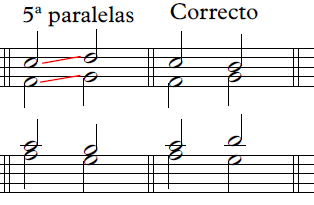
\includegraphics[scale=0.7]{imagenes/5paralelas.png}
		\caption{Ejemplo de quintas paralelas}
		\label{fig2.1.1}
	\end{figure}

	\item \textit{Quintas directas}: dadas dos voces, éstas no pueden producir un intervalo de quinta por movimiento directo.

	\begin{figure}[H]
		\centering
		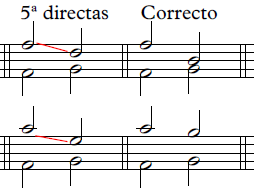
\includegraphics[scale=0.7]{imagenes/5directas.png}
		\caption{Ejemplo de quintas directas}
		\label{fig2.1.2}
	\end{figure}

	\item \textit{Octavas paralelas}: dadas dos voces, éstas no pueden producir dos intervalos de octava consecutivos. 

	\begin{figure}[H]
		\centering
		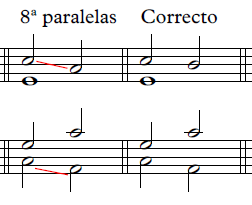
\includegraphics[scale=0.7]{imagenes/8paralelas.png}
		\caption{Ejemplo de octavas paralelas}
		\label{fig2.1.3}
	\end{figure}

	\item \textit{Octavas directas}: dadas dos voces, éstas no pueden producir un intervalo de octava por movimiento directo.

	\begin{figure}[H]
		\centering
		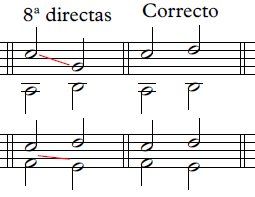
\includegraphics[scale=0.7]{imagenes/8directas.png}
		\caption{Ejemplo de octavas directas}
		\label{fig2.1.4}
	\end{figure}

	\item \textit{Tritono}: dadas dos voces, éstas no pueden producir un intervalo de cuarta aumentada o tritono. No obstante, si éste viene preparado por movimiento conjunto u oblicuo de las voces no se considerará falta.

	\begin{figure}[H]
		\centering
		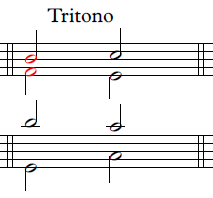
\includegraphics[scale=0.7]{imagenes/tritono.png}
		\caption{Ejemplo de cuarta aumentada}
		\label{fig2.1.5}
	\end{figure}

	\item \textit{Duplicación de sensible}: en ningún caso se podrá duplicar la sensible de la tonalidad. 

	\begin{figure}[H]
		\centering
		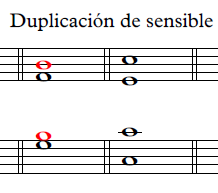
\includegraphics[scale=0.7]{imagenes/sensibledup.png}
		\caption{Ejemplo de duplicación de sensible}
		\label{fig2.1.6}
	\end{figure}

	\item \textit{Búsqueda de acordes incompletos}: todos los acordes deberán de tener la fundamental, la tercera y la quinta del acorde en al menos una voz, especialmente si están invertidos. No obstante, se puede dar la situación de que el acorde de tónica quede incompleto, con la ausencia de la quinta, en la cadencia.

	\item \textit{Segunda inverión consecutiva}: en ningún caso podrá haber dos acordes en segunda inversión consecutivos.

	\item \textit{Lógica tonal}: la armonía de la obra deberá seguir, en la medida de lo posible, el esquema indicado en la figura .

		\begin{itemize}

			\item La tónica o primer grado (I) podrá moverse hacia cualquier otro grado de la escala.
			\item La supertónica o segundo grado (II) podrá moverse hacia el cuarto, quinto o séptimo grado.
			\item La mediante, modal o tercer grado (III) podrá moverse hacia sexto grado.
			\item La subdominante o cuarto grado (IV) podrá moverse hacia el segundo, quinto o séptimo grado.
			\item La dominante o quinto grado (V) podrá moverse hacia el primer, sexto o séptimo grado.
			\item La superdominante o sexto grado (VI) podrá moverse hacia el segundo o cuarto grado.
			\item La subtónica o séptimo grado (VII) podrá moverse hacia el primer, tercer o quinto grado.
		\end{itemize}

		\begin{figure}[H]
			\centering
			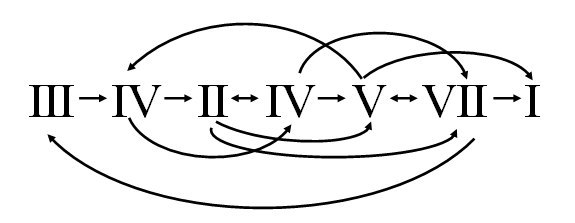
\includegraphics[scale=0.7]{imagenes/logica.jpg}
			\caption{Diagrama de lógica tonal}
			\label{fig2.1.7}
		\end{figure}

		Por otra parte, no podrán darse en ningún caso las siguientes sucesiones de acordes:

		\begin{itemize}
			\item I-II en estado fundamental.
			\item II-III en estado fundamental,
			\item III-IV en estado fundamental.
		\end{itemize}

\end{itemize}

\bigskip

La realización del análisis melódico implica la comprobación de los siguientes hechos:

\begin{itemize}

	\item \textit{Resolución de sensibles}: la sensible de la tonalidad deberá resolver siempre en la tónica.

	\begin{figure}[H]
		\centering
		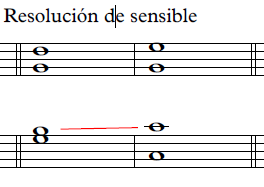
\includegraphics[scale=0.7]{imagenes/sensibleres.png}
		\caption{Ejemplo sensible sin resolver}
		\label{fig2.1.8}
	\end{figure}

	\item \textit{Resolución de séptimas}: la séptima de dominante deberá resolver siempre por movimiento por grado conjunto descendente y deberá estar preparada.

	\begin{figure}[H]
		\centering
		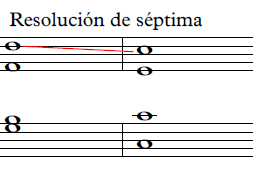
\includegraphics[scale=0.7]{imagenes/septimares.png}
		\caption{Ejemplo de séptima de dominante sin resolver}
		\label{fig2.1.9}
	\end{figure}

	\item \textit{Segunda aumentada}: en ningún caso podrá haber un intervalo de segunda aumentada entre dos notas consecutivas en una misma voz.

	\begin{figure}[H]
		\centering
		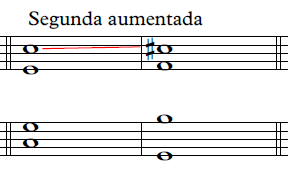
\includegraphics[scale=0.7]{imagenes/2aumentada.png}
		\caption{Ejemplo de segunda aumentada melódica}
		\label{fig2.1.10}
	\end{figure}

	\item \textit{Tritono melódico}: en ningún caso podrá haber un intervalo de cuarta aumentada o tritono entre dos notas consecutivas en una misma voz.

	\begin{figure}[H]
		\centering
		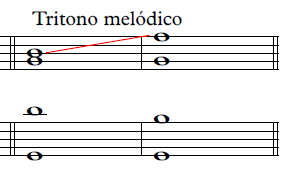
\includegraphics[scale=0.7]{imagenes/tritonomel.png}
		\caption{Ejemplo de cuarta aumentada melódica}
		\label{fig2.1.11}
	\end{figure}

	\item \textit{Contrapunto en voces extremas}: deberá predominar el movimiento contrario en las voces extremas sobre el movimiento oblicuo y, especialmente, directo.

	\item \textit{Contrapunto del salto}: si hay dos movimientos (saltos) en la misma dirección, ascendente o descendente, la primera y la última nota no pueden ser disonantes.

	\item \textit{Melodía incoherente}: deberá predominar el movimiento por grados conjuntos en las melodías, evitando hacer demasiados saltos.

\end{itemize}

\bigskip
\bigskip

En base a todas estas reglas los requisitos funcionales sería los siguientes:

\textbf{RF-1.}Análisis armónico. \\
El sistema llevará cabo un análisis sobre la armonía y los acordes de la partitura en busca de faltas y errores en las secuencias armónicas.

\begin{itemize}

	\bigskip
	\item \textbf{RF-1.1.} Se realizará la búsqueda de quintas paralelas.

	\bigskip
	\item \textbf{RF-1.2.} Se realizará la búsqueda de quintas directas.

	\bigskip
	\item \textbf{RF-1.3.} Se realizará la búsqueda de octavas paralelas.

	\bigskip
	\item \textbf{RF-1.4.} Se realizará la búsqueda de octavas directas.

	\bigskip
	\item \textbf{RF-1.5.} Se realizará la búsqueda de tritonos o cuartas aumentadas.

	\bigskip
	\item \textbf{RF-1.6.} Se realizará la búsqueda de sensibles duplicadas.

	\bigskip
	\item \textbf{RF-1.7.} Se realizará la búsqueda de acordes incompletos.

	\bigskip
	\item \textbf{RF-1.8.} Se realizará la búsqueda de secuencias de acordes en segunda inversión consecutivos.

	\bigskip
	\item \textbf{RF-1.9.} Se realizará una comprobación sobre las secuencias de acordes para asegurar que siguen las reglas de la lógica tonal.

\end{itemize}

\bigskip
\textbf{RF-2.} Análisis melódico.\\
El sistema llevará a cabo un análisis sobre las melodías de las voces en busca de una mala conducción de éstas o de un mal uso del contrapunto.

\begin{itemize}

	\bigskip
	\item \textbf{RF-2.1.} Se comprobará la resolución de sensibles en la tónica.

	\bigskip
	\item \textbf{RF-2.2.} Se comprobará la resolución de todas las séptimas de dominante.

	\bigskip	
	\item \textbf{RF-2.3.} Se comprobará la existencia de intervalos de segunda aumentada melódicos.

	\bigskip
	\item \textbf{RF-2.4.} Se comprobará la existencia de tritonos o intervalos de cuarta aumentada melódicos.

	\bigskip
	\item \textbf{RF-2.5.} Se comprobará la existencia de un buen contrapunto entre las voces de la soprano y del bajo.

	\bigskip
	\item \textbf{RF-2.6.} Se comprobará la existencia de saltos consecutivos con disonancias.

	\bigskip
	\item \textbf{RF-2.7.} Se comprobará la existencia de una buena praxis en las líneas melódicas. 

\end{itemize}

\subsection{Requisitos no funcionales}

Los requisitos no funcionales son aquellos referidos al desarrollo pero no necesariamente relacionados con la funcionalidad del sistema, como aspectos referidos a la interfaz, al rendimiento o a la fiabilidad del sistema.

\bigskip
\textbf{RNF-1.} Los usuarios del sistema deberán estar familiarizados con el lenguaje específico empleado en el ámbito musical para poder entender las explicaciones aportadas por el sistema.

\textbf{RNF-2.} Las pruebas y validaciones del sistema se llevarán a cabo por uno de los expertos.

\section{Modelos de casos de uso}

\subsection{Descripción básica de los actores}

\begin{table}[H]
	\begin{tabular}{@{}|l|p{9cm}|p{2cm}|@{}}
		\hline
		\textbf{Actor}  & Ingeniero del conocimiento & \cellcolor[HTML]{C0C0C0}ACT-1  \\ \hline
		\textbf{Descripción} & \multicolumn{2}{p{11cm}|}{Ingeniero encargado del proceso de adquisición de conocimiento y creación del sistema} \\ \hline
		\textbf{Características} & \multicolumn{2}{p{11cm}|}{Es también el desarrollador que lleva a cabo la implementación del sistema.} \\ \hline
		\textbf{Relaciones} & \multicolumn{2}{p{11cm}|}{ACT-2, ACT-3} \\ \hline
		\textbf{Referencias} & \multicolumn{2}{p{11cm}|}{} \\ \hline
	\end{tabular}
	\caption{Descripción del actor Ingeniero del Conocimiento}
	\label{tablaACT1}
\end{table}

\begin{table}[H]
	\begin{tabular}{@{}|l|p{9cm}|p{2cm}|@{}}
		\hline
		\textbf{Actor} & Experto & \cellcolor[HTML]{C0C0C0}ACT-2 \\ \hline
		\textbf{Descripción} & \multicolumn{2}{p{11cm}|}{Persona a la que el ingeniero del conocimiento entrevista para conocer el ámbito del problema y los procedimientos necesarios para su resolución} \\ \hline
		\textbf{Características} & \multicolumn{2}{p{11cm}|}{Persona experta en el ámbito del problema a resolver por el sistema experto.} \\ \hline
		\textbf{Relaciones} & \multicolumn{2}{p{11cm}|}{ACT-1} \\ \hline
		\textbf{Referencias} & \multicolumn{2}{p{11cm}|}{} \\ \hline
	\end{tabular}
	\caption{Descripción del actor Experto}
	\label{tablaACT2}
\end{table}

\begin{table}[H]
	\begin{tabular}{@{}|l|p{9cm}|p{2cm}|@{}}
		\hline
		\textbf{Actor} & Usuario & \cellcolor[HTML]{C0C0C0}ACT-3 \\ \hline
		\textbf{Descripción} & \multicolumn{2}{p{11cm}|}{Usuario final al que está dirigido el sistema} \\ \hline
		\textbf{Características} & \multicolumn{2}{p{11cm}|}{El usuario, al igual que el experto, tendrá algunos conocimientos sobre el dominio del problema} \\ \hline
		\textbf{Relaciones} & \multicolumn{2}{p{11cm}|}{ACT-1} \\ \hline
		\textbf{Referencias} & \multicolumn{2}{p{11cm}|}{} \\ \hline
	\end{tabular}
	\caption{Descripción del actor Usuario}
	\label{tablaACT3}
\end{table}

\subsection{Descripción de casos de uso}

\begin{table}[H]
	\begin{tabular}{@{}|l|p{9cm}|p{2cm}|@{}}
		\hline
		\textbf{Caso de uso} & Analizar partitura & \cellcolor[HTML]{C0C0C0}CU-1 \\ \hline
		\textbf{Actores} & \multicolumn{2}{p{11cm}|}{Usuario} \\ \hline 
		\textbf{Tipo} & \multicolumn{2}{p{11cm}|}{Primario, esencial.} \\ \hline
		\textbf{Referencias} & \multicolumn{2}{p{11cm}|}{RI-1,RI-2,,RI-3,RI-4,RI-5,RF-1,RF-2} \\ \hline
		\textbf{Precondición} & \multicolumn{2}{p{11cm}|}{Partitura almacenada en el servidor y opciones seleccionadas enviadas} \\ \hline
		\textbf{Postcondición} & \multicolumn{2}{p{11cm}|}{Se crearán archivos con los resultados del análisis para mostrarse a través de la interfaz.} \\ \hline
		\textbf{Propósito} & \multicolumn{2}{p{11cm}|}{Realización del análisis deseado en la partitura aportada por el usuario y obtenicón de resultados.} \\ \hline
		\textbf{Resumen} & \multicolumn{2}{p{11cm}|}{Una vez se han propocionado todos los datos necesarios, el usuario podrá activar el sistema para obtener la lista de errores y faltas encontrados en su partitura para su posterior corrección.} \\ \hline
	\end{tabular}
	\caption{Descripción del caso de uso CU-1}
	\label{CU-1}
\end{table}

\begin{table}[H]
	\begin{tabular}{@{}|p{7.1cm}|p{7.1cm}|@{}}
		\hline
		\multicolumn{2}{|c|}{\textbf{Curso normal}}\\ \hline
		{Accion del actor} & {Acción del sistema} \\ \hline
		(1) Usuario: selecciona las opciones de análisis propuestas por el sistema. & \\ \hline
		 & (2) Sistema: comprueba las opciones seleccionadas. \\ \hline 
		(3) Usuario: selecciona el archivo de la partitura y lo sube al servidor del sistema. &  \\ \hline
		 & (3) Sistema: comprueba el archivo adjuntado.  \\ \hline 
		(5) Usuario: envía los datos al sistema. & \\ \hline
		 & (6) Sistema: almacena las opciones seleccionadas por el usuario.  \\ \hline
		 & (7) Sistema: almacena la partitura en el servidor.  \\ \hline
		 & (8) Sistema: lanza los módulos de análisis seleccionados.  \\ \hline
		 & (9) Sistema: obtiene los resultados de los módulos. \\ \hline
		 & (10) Sistema: muestra los resultados de los módulos. \\ \hline
	\end{tabular}
	\caption{Descripción del curso normal del caso de uso CU-1}
	\label{CNCU-1}
\end{table}

\begin{table}[H]
	\begin{tabular}{@{}|p{14.7cm}|@{}}
		\hline
		\textbf{Cursos alternos}\\ \hline
		(2a) El usuario no ha seleccionado ninguna opción. \\ 
		\hspace{1.5cm}Sistema: informa del error y vuelve a solicitar la selección de opciones. \\
		(4a) El usuario no ha seleccionado ningún archivo. \\
		\hspace{1.5cm}Sistema: informa del error y vuelve a solicitar la selección de un archivo. \\
		(4b) El usuario ha seleccionado un archivo no válido. \\
		\hspace{1.5cm}Sistema: informa del error y vuelve a solicitar la selección de un archivo válido. \\ \hline
	\end{tabular}
	\caption{Descripción de los cursos alternos del caso de uso CU-1}
	\label{CACU-1}
\end{table}

%\section{Diagramas de casos de uso}

%\begin{figure}[H]
%	\centering
%	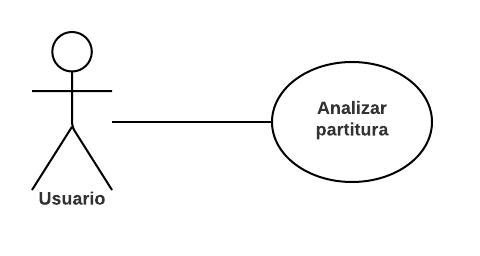
\includegraphics[scale=0.7]{imagenes/casoUso.png}
%	\caption{Diagrama de casos de uso}
%	\label{fig2.4.1}
%\end{figure}

\section{Diagramas de actividad}

\begin{figure}[H]
	\centering
	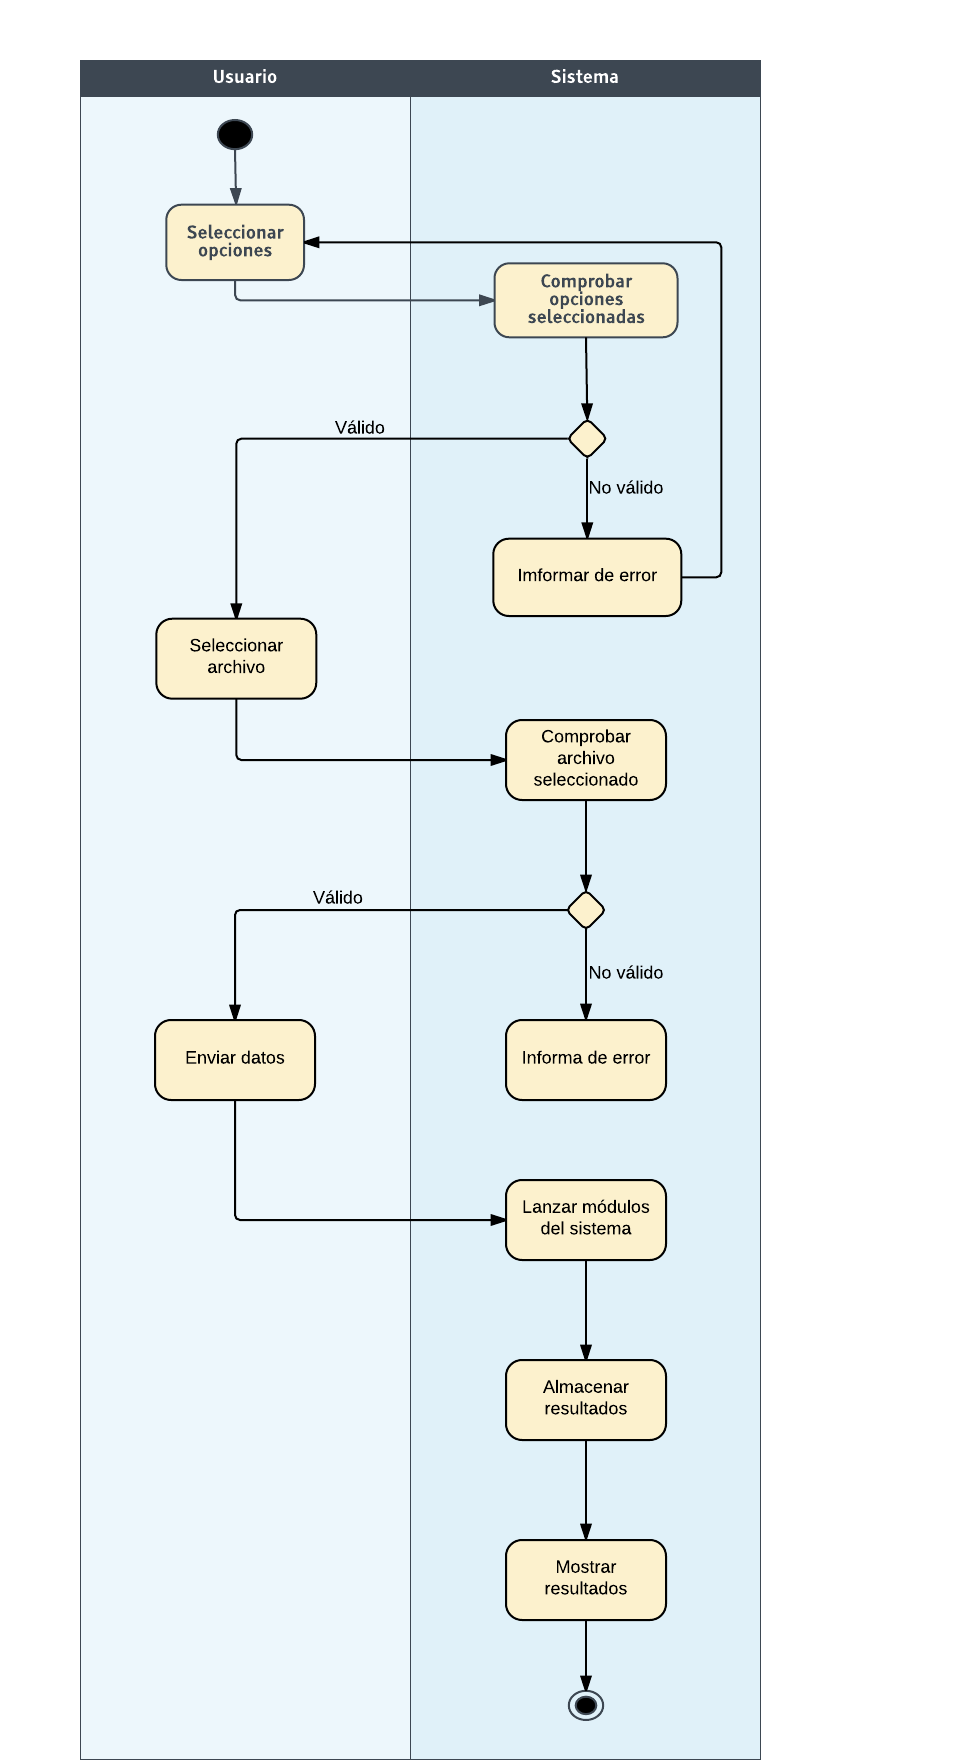
\includegraphics[scale=0.65]{imagenes/diagramaAct.png}
	\caption{Diagrama de actividad del caso de uso CU-1. Analizar partitura.}
	\label{fig2.5.1}
\end{figure}